\chapter{Introduction}
\label{chap: intro}
Remanufacturing has increasingly received attention because of its energy-saving, eco-friendly, and cost-efficient characteristics. Remanufactured products have been presented in automotive, aerospace, and industrial machinery industries. For example, in the automotive industry, companies have been recycling and remanufacturing components such as engine, transmission, car body, etc., as a long-term tradition. In short, remanufacturing is a process of returning a used product to at least original performance specification from the customers’ perspective \cite{remanufacturing-IJOMAH2004}. To achieve this, secondary materials screening for quality control in remanufacturing processes by estimating the quantities of interest, e.g., remaining useful life (RUL) and residual stress, in incoming recycled end-of-life (EoL) products becomes an essential step and is crucial in increasing the usage of recycled materials. 

In recycled components, material fatigue damage is universally presented and it is one of the most influential factors that determine the RUL of a used product. Material fatigue has resulted in many catastrophic accidents in the history and has been studied for many decades; however, the fatigue damage level is hard to be monitored in real-world environments due to the stochastic nature of fatigue behaviors and undetermined loading conditions \cite{fatigue-review-Santecchia2016}, which is a critical issue to be addressed.

To quantitatively study fatigue damage in materials, non-destructive evaluation (NDE) methods have been developed \cite{nde-review-ACHENBACH200013,nde-review-WISNER2020}. NDE, also known as non-destructive testing, is a technique to evaluate material properties without causing damage to the testing parts. For instance, linear ultrasonic (LU) 
% \cite{nde-lu-fatigue-JOSHI1972577}
and nonlinear ultrasonic (NLU) testings 
% \cite{nde-nlu-fatigue-NAGY1998375,nde-nlu-review-Matlack2014,nde-nlu-fatigue-Cantrell}
send ultrasonic waves which propagate in a material and then analyze the response signals to evaluate material degradation. Although there exist a variety of NDE techniques 
% \cite{nde-thermo-FAN20121, nde-dic, nde-microwave, nde-magnetic, nde-ae-CHAI2017101,nde-electrical-resistance-SUN2007}
, each of these methods is only sensitive to a few specific fatigue conditions and is limited to detecting defects in certain length scales. For example, LU testing is robust at detecting macro-scale defects; in contrast, NLU techniques measure nonlinear material parameters to detect defects that are orders of magnitude smaller than the probing wavelength (e.g., typically on the order of 1 mm stainless steels), providing an important data source of early-stage damage characterization.

% \begin{figure}[tb]
%     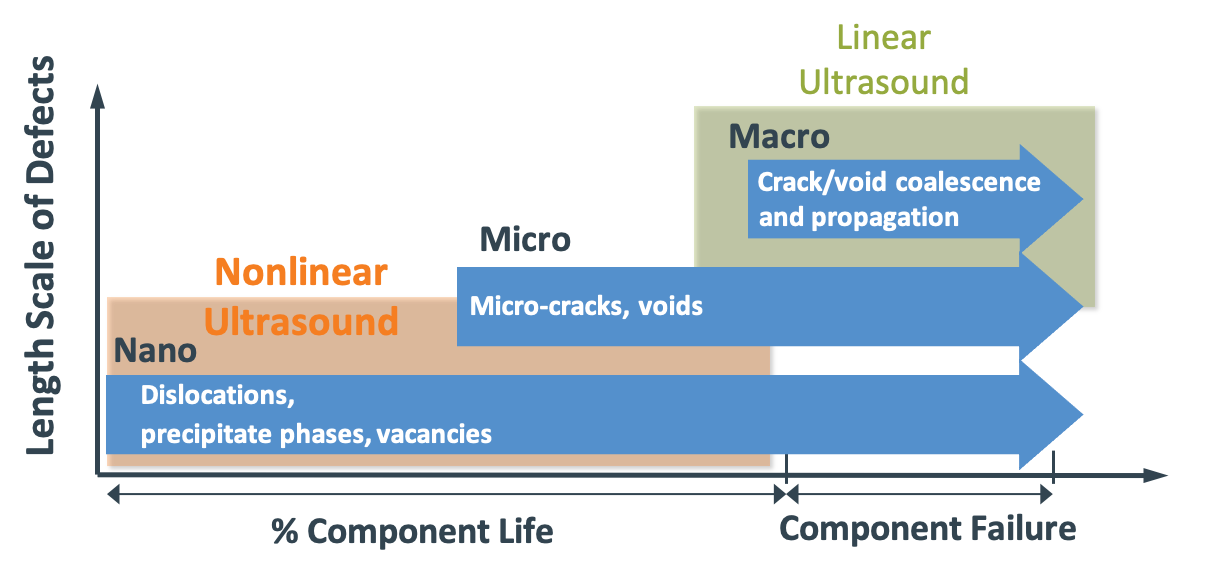
\includegraphics[width=\linewidth]{fig/lu_nlu_length_scales.png}
%     \caption{Capability of defect detection for LU and NLU testings}
%     \label{fig: lu nlu length scales}
% \end{figure}

There is a lack of research on the estimation and prognosis of RUL of EoL components in the remanufacturing industry even though, with state-of-the-art machine learning (ML) models, RUL estimation has been successfully applied in many industrial components, e.g., bearing \cite{rul-nn-bearing-BENALI2015150, rul-cnn-bearing-LI20181, rul-ensemble-bearing}, gear \cite{rul-review-gear}, turbofan engine \cite{rul-statespace-turbo-battery-Mosallam2016,rul-cnn-turbo-LI20181,rul-rnn-turbo-WU2020241}, and lithium-ion battery \cite{rul-statespace-turbo-battery-Mosallam2016,rul-review-battery-LIPU2018115,rul-gpr-battery-9040661}. Unlike the examples in the literature, the possible difficulties for RUL estimation in remanufacturing are as follows. First, continuous and in-situ measurements are generally not available, i.e., it is impossible to know the historical measurements of a recycled component. Second,
environmental noises can affect the performance of sensing as well as the built algorithms. Third, sufficient data in EoL products or remanufacturing may be hard to collect, introducing difficulties in building robust data-driven models.

In this research, we propose an ML-based NDE methodology for the quantification and prognostics of accumulated fatigue damage in recycled materials. The general idea of this research is illustrated by Figure \ref{fig: general idea}.
\begin{figure}[tb]
    \centering
    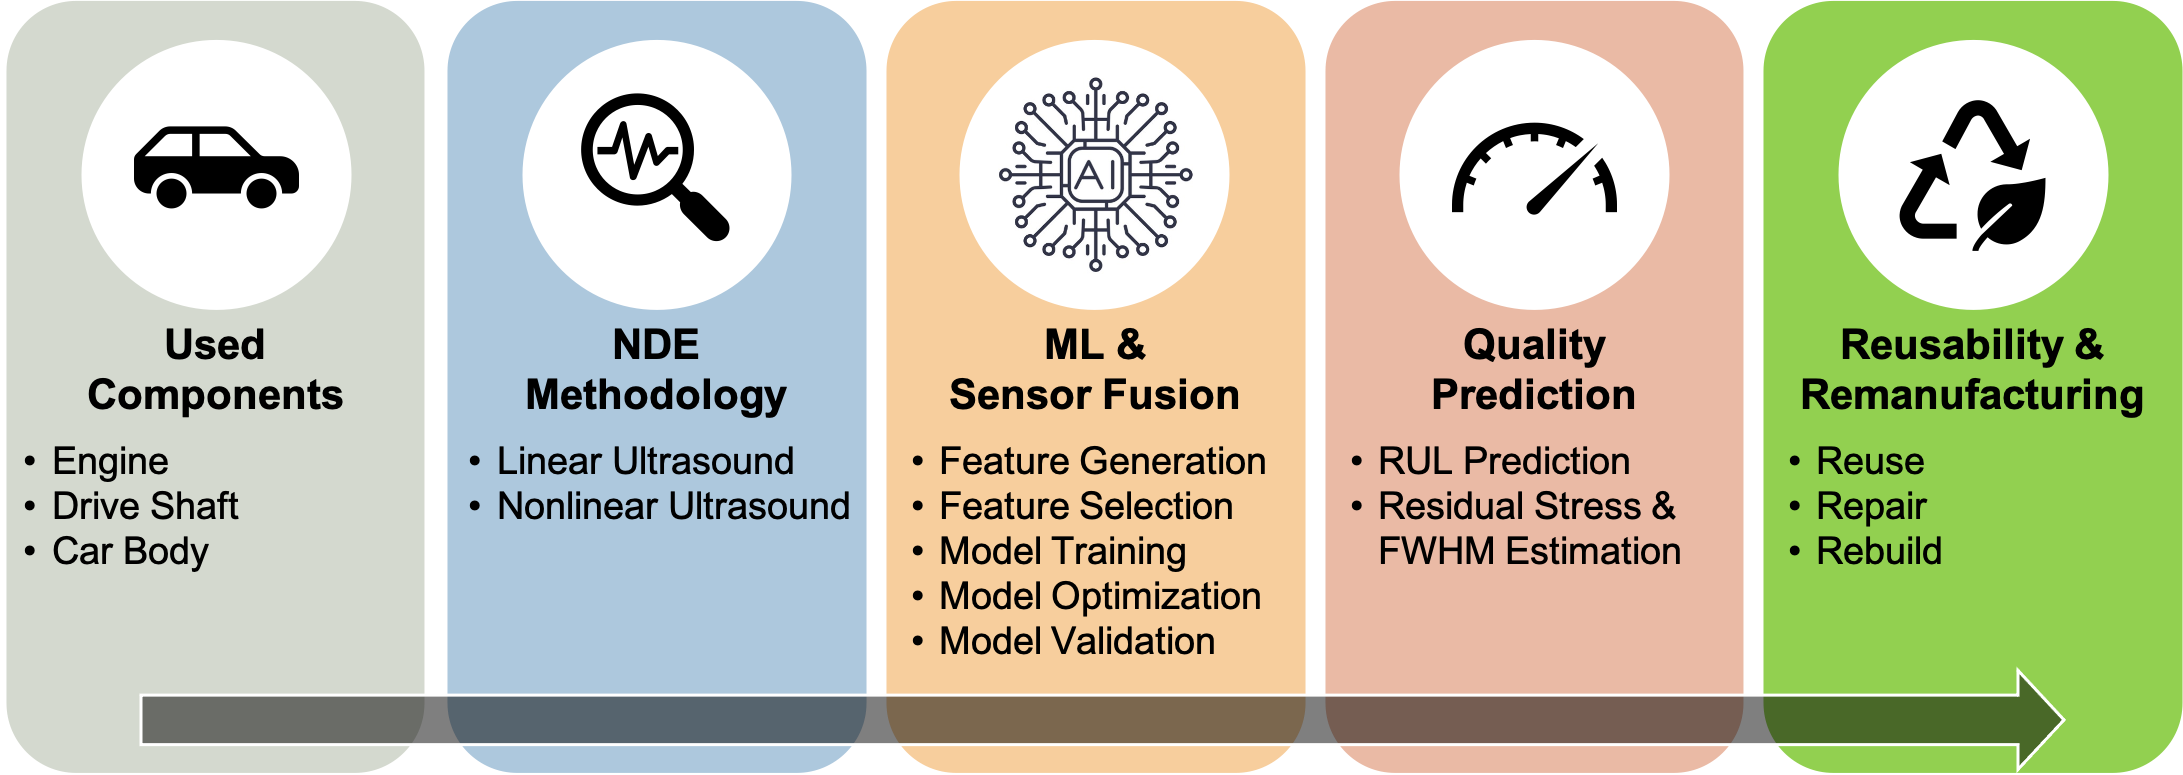
\includegraphics[width=\linewidth]{fig/general_idea.png}
    \caption{General idea of the proposed methodology}
    \label{fig: general idea}
\end{figure}
 First, we integrate LU and NLU testings to leverage the strength of each individual sensor, which has the potential of estimating different fatigue conditions simultaneously.
% \cite{nde-review-WISNER2020}
Second, with multi-output hierarchical classifiers,
%  \cite{hierarchical-Silla2011}
an RUL estimation framework is developed by predicting the loading condition as well as the percentage of fatigue life that a component has undergone, and then the RUL is estimated from an S-N curve. In the proposed approach, both ultrasonic testings serve as ex-situ measurement methods to predict the loading history of a recycled component. Therefore, without continuous monitoring data of a component from its healthy state, the RUL can be inferred by using the current measurement only. Besides, we develop a residual stress measurement method based on the proposed NDE methodology and ML techniques, which shows excellent potential of being an efficient method in terms of test speed and cost.

This research is targeted at metals that are widely used in a number of industry sectors. In this study, the target material is 5052-H32 aluminum alloy which is widely used in truck and auto industries. Life cycle fatigue testings were conducted in different settings to construct a comprehensive database for fatigue progression in the target material. The fatigued specimens were later examined by ultrasonic as well as X-ray diffraction (XRD) measurements. Here, XRD measurements serve as the calibration for residual stress and full width at half maximum (FWHM) estimation. After that, the proposed NDE methodology and prediction framework were developed and tested on the collected fatigued samples.

% The goal of this research is to not only enable effective materials screening but also provide valuable information for the process optimization and control of downstream remanufacturing processes. As such, an effective NDE method that is applicable on the factory floor will lead to greater material recycling and improved quality of products that are produced using recycled materials.

The remainder of this thesis is organized as follows. Chapter \ref{chap: litrev} provides the literature review of the related topics. Chapter \ref{chap: exper} describes the experimental setup and procedures including the design of experiments, life cycle fatigue testing, ultrasonic and XRD measurements. Chapter \ref{chap: model} introduces the ML model development procedure used in both Chapter \ref{chap: rul} and Chapter \ref{chap: reg} where the proposed RUL estimation framework and residual stress measurement method are presented, respectively, with the case study on our fatigue test dataset. Finally, in Chapter \ref{chap: concl}, the contributions of this thesis are summarized and future research directions are discussed.

